% Pensez à indiquer english ici pour gérer les césures correctement
% Merci de ne conserver cette ligne pour éviter que le paramètre ne soit écrasé par un article précédent dans les actes
\selectlanguage{french} % valeurs possibles : french, english

\settitle[Analyse de la sécurité RDP]{RDP: Analyse de la sécurité offerte par NLA}

\setauthor[M.Bourguenolle, M.Bertoli]{Thomas Bourguenolle\inst{1} \and Geoffrey Bertoli\inst{2}\\
  \email{contact@croustibaie.fr\\contact@bertoli.me}}

\institute{EY \and Synacktiv}

% Pour gérer des organismes d'appartenance multiples, voici le modèle:
%
%   \setauthor[M.~MonNom, A.~MonAutreNom]{MonPrenom MonNom\inst{1} \and AutrePrenom AutreNom\inst{2}\\
%     \email{monprenom.monnom@mycorp.com\\autreprenom.autrenom@mycorp.com}}
%
%   \institute{OrganismePourMonNom \and OrganismePourAutreNom}
%
% Dans \institute, la numérotation se fera automatiquement et commence à 1


\maketitle
\index{Bourguenolle, M.}
\index{Bertoli, M.}

\begin{abstract}
RDP est un protocole d'administration à distance, sa prédominance dans les environnements Windows en fait une cible de choix pour les attaquants.RDP en est actuellement à la version 10.5 et supporte diverses mesures de sécurité pour se protéger notamment des attaques de type "man in the middle".

Les auteurs ont souhaité étudier les possibilités de réalisation de telles attaques, notamment dans le cadre d'une connexion réalisée avec le mécanisme NLA. La suite du document présente une analyse du niveau de sécurité réellement apporté par NLA et un outil ayant été développé pour mettre en place des scénarios d'attaque de type "man in the middle" sur des connexions NLA.
\end{abstract}


\section{Introduction}

\subsection{État de l'art}
Les serveurs RDP supportent actuellement 3 modes d'authentification distincts pour l'éblissement d'une connexion:
\begin{itemize}
\item \textbf{RDP Standard Security}: Les échanges entre le client et le serveur sont chiffrés à l'aide d'une clé symétrique. Cette clé est négociée à partir d'un échange RSA établi avec une paire de clés fixe spécifié dans la documentation Microsoft. La mise en place d'une attaque de type MiTM est donc triviale dans ce cas.
\item \textbf{RDP Enhanced sécurity TLS} (Depuis RDP 5.2): Les échanges entre le client et le serveur sont chiffrés à l'aide d'une clé symétrique négociée dans un canal TLS. Les attaques de type Man-In-The-Middle nécessitent donc de posséder un certificat valide au sein de l'infrastructure Windows ou d'obtenir l'accord du client suite à l'affichage du message d'erreur indicant l'invalidité du certificat.  
\item \textbf{DP Enhanced security NLA} (Depuis RDP 6.0): Mode d'authentification par défaut depuis Windows Server 2012R2. Dans ce mode, l'utilisateur réalise l'authentification dès l'ouverture de la session RDP, la mire d'authentification Windows n'est donc pas affichée à l'utilisateur. Lors de l'authentification, les échanges entre le client et le serveur sont chiffrés à l'aide d'une clé symétrique négociée dans un canal TLS après « authentification mutuelle » des deux acteurs (via Kerberos ou NTLMSSP). En pratique, l'implémentation de NLA est réalisée par CredSSP. Les attaques de type Man-In-the Middle semblent difficiles à mettre en place notamment lorsque l’authentification mutuelle est effectuée via Kerberos.
\end{itemize}

Les outils suivants permettent l'implémentation de certains scénarios de "man in the middle" sur des connexions RDP:

L’outil SETH (https://github.com/SySS-Research/Seth) présenté à Hackitivity 2017 offre la possibilité de dégrader une connexion RDP Enhanced Security NLA vers RDP Enhanced Security. Pour ce faire, l’outil bloque les requêtes Kerberos du client puis annonce une indisponibilité du DC. Suite à cela, un certificat non valide est présenté au client dans le but d’intercepter les authentifiants de la victime dans le cas où celle-ci accepterait l’établissement de la connexion malgré le message d'erreur. Il n’existe à l’heure actuelle aucun moyen de forcer l’utilisation de RDP Enhanced security NLA cotée client, cette attaque est donc toujours réalisable.

L'outil PyRDP présenté (https://github.com/gosecure/pyrdp) en aout 2019 à BlackHat Arsenal, permet de générer dynamiquement un certificat autosigné au nom du serveur cible afin de réaliser une attaque de Man-in-the-middle sur des environnements utilisant le mode d'authentification RDP Enhanced Security TLS. L'outil permet l'enregistrement de session, l'injection de commande, le rejeu, ainsi que la capture d'entrée utilisateur et donc de secret d'authentification. Néanmoins cet outil ne supporte pas le mode d'authentification NLA.

Le succès des attaques déployées avec ces outils reposent sur l'acceptation de l'erreur de certificat par l'utilisateur. Ce type d'attaque dispose de grandes chances de succès si les utilisateurs sont habitués à accepter le message d'erreur dû à l'invalidité du certificat. Ce genre de situation peut se produire si aucune PKI n'a été déployée ou si les utilisateurs initient leurs connexions RDP en spécifiant l'adresse IP du serveur de destination et que cette adresse n'a pas été ajoutée aux noms alternatifs du certificat.

Aucun des outils existant à l’heure actuelle ne gère le mode d’authentification RDP Enhanced Security NLA, même si Seth possède un moyen de dégrader l’authentification. Depuis la vulnérabilité CVE-2019-0708, les recommandations de Microsoft sont, côté serveur, de n’accepter que les connexions réalisées via RDP Enhanced Security NLA, diminuant considérablement l'utilité des outils actuels.

L'article Sécurité de RDP par Aurélien BORDES, Arnaud EBALARD et Raphaël RIGO présente, entre autres, les différents modes authentifications RDP et précise en quoi une attaque de type MiTM sur NLA reste possible moyennant la compromission d'un compte machine dans le domaine cible. 

En initiant le développement d’un outil permettant d’effectuer des attaques de type Man-In-The-Middle supportant l’authentification NLA, les auteurs ont pu constater certains problèmes liés à ce mode d’authentification. Ce document présente ces faiblesses et expose en quoi l’utilisation de NLA pourrait mettre l’ensemble de l’infrastructure plus à risque qu’avec l’utilisation de RDP Enhanced Security TLS.
Ces vulnérabilités permettent notamment la récupération de réponse NTLMv2 de manière transparente pour la victime même dans le cas où celle-ci appartient au groupe "Protected Users".

\section{Analyse des connexions NLA}
\subsection{Comment fonctionne l'authentification NLA}
Une authentification via NLA se déroule comme suit :

% Exemple d'inclusion d'une figure
% (avec une version couleur)

\begin{figure}[ht]
  \centering
  \ifssticbw
    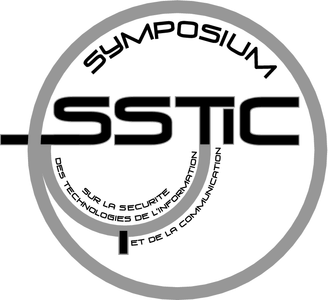
\includegraphics[width=0.4\textwidth]{MonNom/img/bw-archi}
  \else
    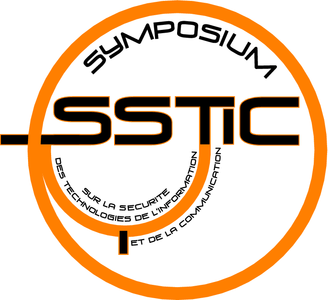
\includegraphics[width=0.4\textwidth]{MonNom/img/archi}
  \fi
  \caption{Légende de l'image}
  \label{fig:monnom:archi}
\end{figure}

Les 4 premières étapes consistent permeetent l'tablissement d'une connexion TLS entre le client et le serveur. Cependant à la différence d’une authentification utilisant RDP Enhanced Security TLS, la validité du certificat n’est ici pas vérifiée. En effet le protocole CREDSSP devant permettre une authentification mutuelle du client et du serveur, la validité du certificat est à priori optionnelle.
Les étapes 5 et 6 servent à négocier le SSP (Security Support Provider) utilisé par la suite, les choix étant NTLMSSP et Kerberos.
\begin{itemize}
	\item NTLMSSP est choisi si le client n’appartient pas à un domaine ou s'il utilise l’adresse IP du serveur pour sy connecter (Kerberos ne fonctionnant qu'avec des FQDN).
	\item Kerberos est choisi lorsque le client appartient au même domaine que le serveur et que le client utilise le FQDN de la cible pour s'y connecter.
\end{itemize}
Les étapes 7 et 8 servent à effectuer l’authentification mutuelle des deux acteurs.
Une fois que l'authentification mutuelle est réalisée, le client envoi ses authentifiants (mot de passe ou smartcard) au serveur lors de l'étape 9. Il est important que de garder à l'esprit que l'objectif final de CredSSP est d'effectuer une délégation des authentifiants du client à un service de confiance. 

\subsection{La structure TSRequest}
Les échanges CredSSP sont réalisés via la structure TSRequest pour réaliser l'authentification mutuelle.

\begin{lstlisting}[frame=single,basicstyle=\tiny]
TSRequest :== SEQUENCE {
	Version     [0] INTEGER,
	negoToken   [1] NegoData OPTIONNAL,
	authInfo    [2] OCTET STRING OPTIONNAL,
	pubKeyAuth  [3] OCTET STRING OPTIONNAL,
	errorCode   [4] OCTET STRING OPTIONNAL,
	clientNonce [5] OCTET STRING OPTIONNAL
	}
\end{lstlisting}


\begin{itemize}
	\item Version: Indique la version du protocole à utiliser. Depuis la vulnérabilité CVE-2018-0886, les clients sont censés refuser les versions 5 et inférieures de CredSSP. Cependant il a été constaté que depuis l’update d’octobre 2019, la version 2 de CredSSP peut de nouveau être utiliséé, réintroduisant potentiellement une vulnérabilité de type Remote Code Execution (mais des analyses sont encore nécessaires de notre part). La suite de ce document considérera une utilisation de la version 6 du protocole.
	\item NegoToken: Contient les jetons permettant la négociation du mode d'authentification à utiliser (NTLMSSP ou kerberos) ainsi que l'authentification en elle-même.
	\item AuthInfo: Contient les authentifiants du client à transmettre au SSP une fois l'authentification mutuelle réalisée. 
	\item pubKeyAuth: Ce champ est utilisé par le client pour envoyer le certificat observé lors de la connexion TLS. Ce certificat sera signé à l'aide d'une clé dérivable à partir des authentifiants du client si NTLMSSP est utilisé, ou bien à l'aide de la clé insérée dans le TGS Kerberos. 
	\item ErrorCode: Utilisé pour transmettre le détail des erreurs rencontrées.
	\item clientNonce: Nonce cryptographique utilisé lors de la signature du certificat dans le champ "pubKeyAuth".
\end{itemize}

\section{Analyse d'une connexion NLA utilisant NTLMSSP}

Etape 5: Le client envoie la requête suivante:

\begin{lstlisting}[frame=single,basicstyle=\tiny]
TSRequest {
	Version:     6,
	negoToken:   NegoData-> NTLMSSPType1Message
	}
\end{lstlisting}

Le message NTLMSSPType1 contient des informations nécessaires pour l’établissement d’un échange NTLMSSP, ainsi que notamment des informations sur la version de NTLMSSP et les paramétrages souhaités par le client.

Étape 6: Le serveur répond comme suit:

\begin{lstlisting}[frame=single,basicstyle=\tiny]
TSRequest {
	Version:     6,
	negoToken:   NegoData-> NTLMSSPType2Message
	}
\end{lstlisting}


Le message NTLMSSPType2 contient les informations de challenge NTLM : NTLMChallenge, Nom du serveur, Nom du domaine

Étape 7 :
Le client envoi maintenant la réponse NTLMv2 ainsi qu'une signature du certificat TLS présenté afin d'initer l'authentification mutuelle :

\begin{lstlisting}[frame=single,basicstyle=\tiny]
TSRequest {
	Version:     6,
	negoToken:   NegoData-> NTLMSSPType3Message,
	pubKeyAuth: Signature + encryptedCertificate,
	clientNonce: Octet String
	}
\end{lstlisting}

Le message NTLMSSPType3 contient la réponse au challenge NTLM contenant:
\begin{itemize}
	\item Réponse NTLMv2
	\item Username
	\item Nom de domaine
	\item EncryptedSessionKey: Cette valeur correspond au chiffrement via RC4 d’une RandomSessionKey avec une clé secrète. La clé utilisée pour chiffrer cette RandomSessionKey est un HMACMD5 dérivé de l'empreinte NTLM de l’utilisateur.
\end{itemize}
Le champ pubKeyAuth contient le chiffrement RC4 du SHA256 de (’CredSSP Client-To-Server Binding Hash’ + Nonce + PublicKey du certificat) avec la Clé RandomSessionKey.
Le Nonce est renvoyé dans le champ ClientNonce.

\textbf{À cette étape, un attaquant effectuant une attaque de type Man-In-The-Middle a récupéré une réponse NTLMv2 de sa victime sans lever aucune alerte de sécurité. Cette empreinte peut être cassée ou utilisée pour des attaques de type SMB Relay}
% Exemples de listes  à points

Étape 8: À cette étape, le serveur vérifie le certificat TLS vu par le client puis prouve son identité auprès du client. Pour ce faire, il envoie la requête suivante:

\begin{lstlisting}[frame=single,basicstyle=\tiny]
TSRequest {
	Version:     6,
	pubKeyAuth: Signature + encryptedCertificate,
	}
\end{lstlisting}

Le champ pubKeyAuth contient le chiffrement RC4 du SHA256 de (’CredSSP Server-To-Client Binding Hash’ + Nonce + PublicKey du certificat)) chiffrer avec la RandomSessionKey.
Pour effectuer cette requête, le serveur doit être en connaissance de la RandomSessionKey. Celle-ci est récupérée auprès du Domain Controller. Pour qu’un attaquant puisse mettre en place une attaque de type Man-In-The-Middle, il doit donc être en mesure de récupérer cette RandomSessionKey. Pour cela il lui suffit d’avoir un compte machine valide au sein du domaine.
L’authentification mutuelle effectuée si le SSP choisi est NTLMSSP n’est donc pas une véritable authentification mutuelle et ne permet de s'assurer que de l'appartenance au domaine de la machine ciblée par le client.

Étape 9 :
Contrairement à ce qui été identifié dans le papier de l’ANSSI, Sécurité RDP, il n’est plus possible d’accéder directement à cette étape et donc de collecter les authentifiants du client depuis RDP > 7.0.
En effet au lieu de passer à l’étape 9, l’authentification recommence à l’étape 1. L'unique différence étant que le client va cette fois-ci contrôler la validité du certificat reçu à la fin de l’étape 2. Si le certificat n'est pas valide, l'utilisateur se verra présenter la fenêtre d'erreur de certificat.
NB : Si l’attaquant possède un compte machine, il est facile pour lui d’obtenir un certificat RDP signé par l’autorité de confiance de l’Active Directory (mais pas au nom du serveur cible). L’erreur sera alors un « name mismatch » ce qui est forcément le cas si l’utilisateur a rentré une adresse IP.
Après présentation de l’erreur de certificat, l’authentification recommence et va juste à l’étape 9.
À l’étape 9 le client envoie la requête suivante :

\begin{lstlisting}[frame=single,basicstyle=\tiny]
TSRequest {
	Version:     6,
	authInfo: Signature + cryptedCreds,
	}
\end{lstlisting}


CryptedCreds contient les secrets d’authentifications de l’utilisateur chiffré via RC4 avec la RandomSessionKey.

\section{Analyse d'une connexion NLA utilisant Kerberos}
Dans ce cas il n’est plus possible pour un attaquant en situation de Man-In-The-Middle de découvrir la RandomSessionKey, s’il ne possède pas le bon compte machine. En effet la RandomSessionKey est maintenant envoyée dans le TGS à destination du serveur qu’un attaquant ne pourra pas déchiffrer simplement avec un compte machine.
Cependant il est possible de partiellement downgrader la connexion pour revenir à une connexion utilisant NTLMSSP.

Étape 5 :
Le client envoi maintenant la TSRequest suivante :

\begin{lstlisting}[frame=single,basicstyle=\tiny]
TSRequest {
	Version:     6,
	NegoToken: Kerberos,
	}
\end{lstlisting}


On remarque que le client ne propose que Kerberos. Même si celui-ci supporte NTLMSSP, il ne le propose pas comme option auprès du serveur.

Étape 6: 
Il est tout de même possible pour un attaquant de répondre à l'aide du message malformé suivant afin de downgrader la communication sur NTLMSSP. La TSRequest suivante permet d'obtenir ce résultat :

\begin{lstlisting}[frame=single,basicstyle=\tiny]
TSRequest {
	Version:     6,
	NegoToken: \xa1\x...NTLMSSP\x00\x00...\x0f,
	}
\end{lstlisting}


Cette requête malformée a été obtenue en analysant la réponse d'un serveur ayant été retiré d'un domaine mais dont le FQDN a été inséré manuellement dans le fichier "hosts" du client. Cette réponse est donc la réponse apportée par un serveur incapable de réaliser une connexion NLA via Kerberos.

\begin{figure}[ht]
  \centering
  \ifssticbw
    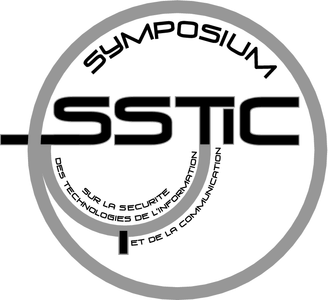
\includegraphics[width=0.4\textwidth]{MonNom/img/bw-archi}
  \else
    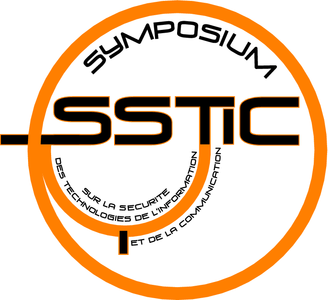
\includegraphics[width=0.4\textwidth]{MonNom/img/archi}
  \fi
  \caption{Légende de l'image}
  \label{fig:monnom:archi}
\end{figure}
\bibliography{MonNom/biblio}

Suite à cette réponse, le client va autoriser la connexion via NTLMSSP mais le protocole n'est plus respecté et la connexion échoue avant sa finalisation.

Étape 5 (bis) :
Le client envoye par la suite un message NTLMSSPType1 mais en l'insérant dans le champ AuthInfo (en lieu et palce du champ NegoToken normalement utilisé):

\begin{lstlisting}[frame=single,basicstyle=\tiny]
TSRequest {
	Version:     6,
	NegoToken: TSRequest{
		Version: 1
		AuthInfo : NTLMSSType1 message
		}
	}
\end{lstlisting}


Étape 6 (bis) :
En respsectant ce "nouveau" mode de fonctionnement, il est possible de répondre de la même manière pour envoyer un message NTLMSSPType2 auprès du client :

\begin{lstlisting}[frame=single,basicstyle=\tiny]
TSRequest {
	Version:     6,
	NegoToken: TSRequest{
		Version: 1
		AuthInfo : NTLMSSType2 message
		}
	}
\end{lstlisting}


Étape 7 :
Le client continue l'échange jusqu'à cette étape et \textbf{va donc envoyer une réponse NTLMSSPType3 contenant la réponse NTLMv2 toujours sans message d’erreur sur le certificat et alors que celui-ci avait forcé l’utilisation de Kerberos. Cette empreinte peut ensuite être cassée ou utilisée pour des attaques de type SMB Relay}

L’absence de valeur dans le champ pubKeyAuth et ClientNonce, empêche l’authentification de terminer. Il n’est donc pas possible d’aller plus loin dans la communication et d’obtenir les authentifiants de la victime en clair comme c’est le cas pour le choix NTLMSSP.

Il est à noter que la victime enverra son empreinte NTLMv2 même si l’utilisateur appartient au groupe « protected users ». En effet d’après Microsoft, cette protection est faite pour protéger un utilisateur authentifié et non un utilisateur en cours d’authentification (bien que les intiations de connexions NTLMSSP soient bloquées sur les autres outils Microsoft...).

\section{Conclusion}
En conclusion l’utilisation obligatoire de NLA sur le réseau semble ajouter plus de risque au sein de l’infrastructure réseau que l’utilisation d’une authentification TLS.
En effet l’absence de vérification du certificat en première instance permet à un attaquant de récupérer une empreinte NTLMv2 sans lever d’alerte, quel que soit le SSP choisi (Kerberos ou NTLMSSP) .
En outre si le SSP utilisé est NTLMSSP alors les « chances » de réussite d’une attaque de type Man-In-The-Middle, sont les mêmes que pour une authentification TLS (acceptation du certificat par la victime) si l’on possède un compte machine au sein du domaine.

Un outil a été développé en python avec la bibliothèque impacket pour réaliser les POC permettant la mise en évidence de ces faiblesses.
En plus de cela l’outil propose une bibliothèque python permettant l’établissement d’une connexion RDP via authentification NLA (coté client et serveur). Cet outil est en cours d’intégration dans un outil plu complet type PyRDP permettant de faire des attaques directement sur RDP (injection de commandes, keylogger etc…)
